Trong phần này, tác giả mô tả một mạng neuron đồ thị tổng hợp metapath mới (MAGNN) để biểu diễn đồ thị không đồng nhất. MAGNN được xây dựng bởi 3 thành phần chính: biến đổi nội dung nút, tổng hợp hợp intra-metapath và tổng hợp inter-metapath. Hình 2 minh họa việc tạo biểu diễn của một nút. Các quá trình lan truyền tiến được chỉ ra trong thuật toán 1.

\subsection{Biến đổi nội dung nút}
Với một đồ thị không đồng nhất liên kết với các thuộc tính nút, các loại nút khác nhau có thể có chiều của các vector đặc trưng không bằng nhau. Kể cả chúng có số chiều bằng nhau thì chúng cũng nằm trên các không gian đặc trưng khác nhau. Ví dụ các bag-of-words vectors $n_1$ chiều của đoạn văn bản và các vectors biểu đồ cường độ $n_2$ chiều của hình ảnh không thể  trực tiếp hoạt động cùng nhau kể cả $n_1 = n_2$. Các vectors đặc trưng với các chiều khác nhau là một khó khăn khi tác giả xử lý chúng trong một framework thống nhất. Do đó, tác giả cần chieus các loại khác nhau của đặc trưng nút vào cùng một không gian vector latent trước.

Vì vậy trước khi đưa các vectors nút vào MAGNN, tác giả áp dụng phép biến đổi tuyến tính cho từng loại nút bằng cách chiếu các vector đặc trưng vào cùng một không gian latent. Với một nút $\nu \in \pmb{\mathcal{V}}_A$ của loại $A \in \pmb{\mathcal{A}}$, ta có
\begin{equation}
  \label{eq:01}
  \mathbf{h'}_{\nu} = \mathbf{W}_A \cdot \mathbf{x}^A_{\nu}
\end{equation}
trong đó $\mathbf{x}_{\nu} \in \mathbb{R}^{d_A}$ là vector đặc trưng gốc và $\mathbf{h'}_{\nu} \in \mathbb{R}^{d'}$ là vector lantent hình chiếu  của nút $\nu$. $\mathbf{W}_A \in \mathbb{R}^{d' \times d_A}$ là ma trận trọng số của các nút loại $A$.

Biến đổi nội dung nút giải quyết tính không đồng nhất của một đồ thị bắt nguồn từ các đặc trưng nội dung nút. Sau khi áp dụng tác động này, tất cả các đặc trưng chiếu của nút đều có cùng chiều, tạo điều kiện thuận lợi cho quá trình tổng hợp của thành phần tiếp theo của mô hình. 

\begin{figure*}
  \label{fig:02}
  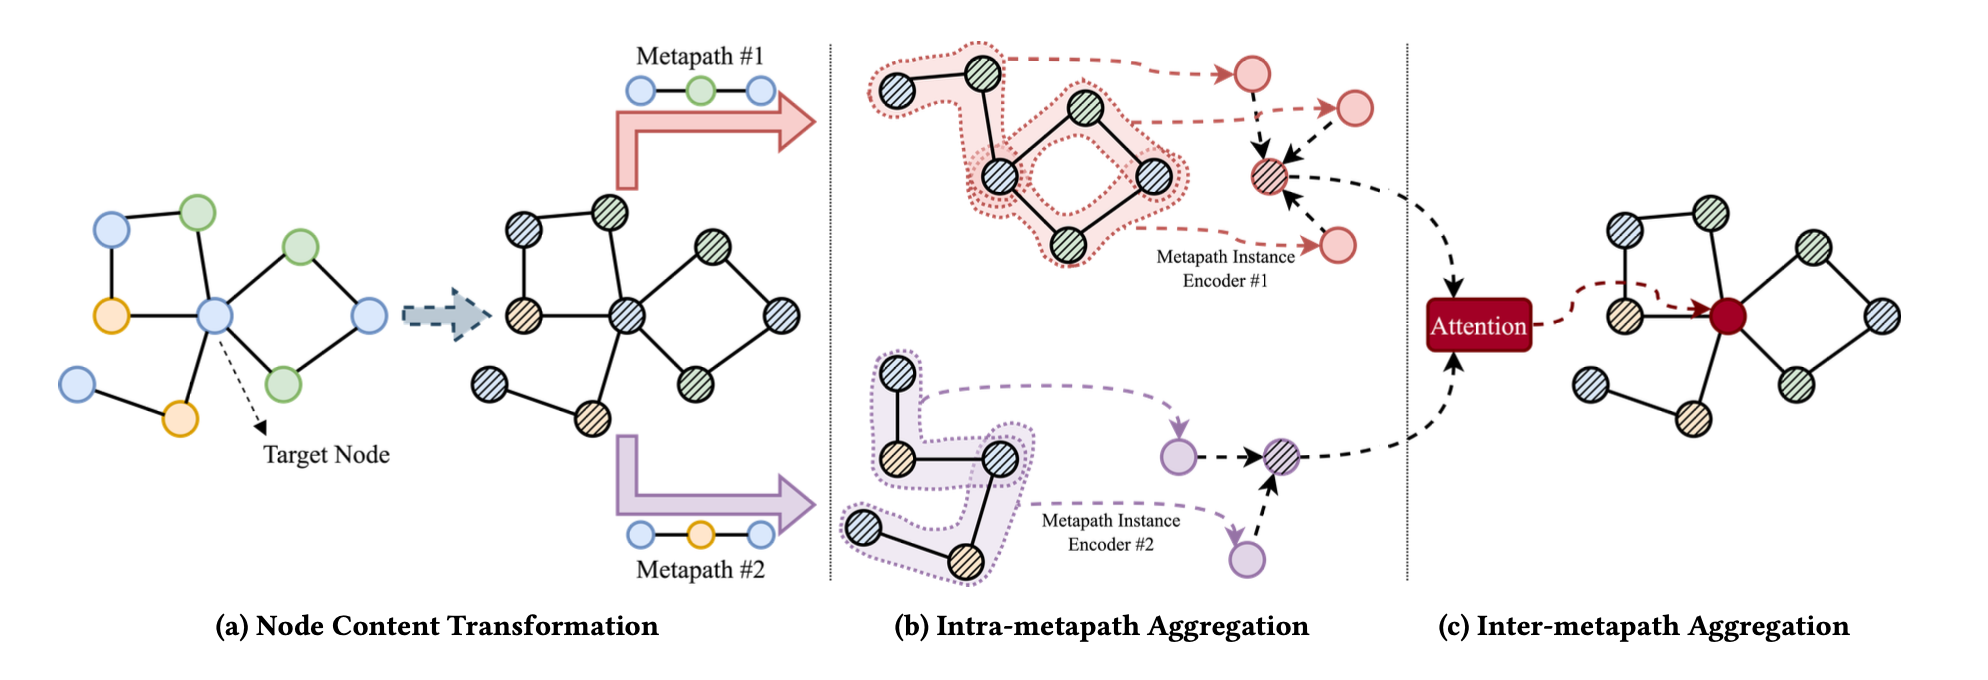
\includegraphics[width=\textwidth]{figs/fig2.png}
  \caption{Kiến trúc tổng thể của MAGNN}
\end{figure*}

\subsection{Tổng hợp intra-metapath}
Cho một metapath $P$, lớp tổng hợp intra-metapath học thông tin cấu trúc và ngữ nghĩa được nhúng trong nút mục tiêu, các lân cận dựa trên metapath và ngữ cảnh ở giữa bằng cách mã hóa cấu hình metapath của $P$. Gọi $P(\nu, u)$ là một cấu hình metapath kết nối nút mục tiêu $\nu$ và lân cận dựa trên metapath $u \in \pmb{\mathcal{N}}^P_{\nu}$, tác giả định nghĩa thêm  nút trung gian của $P(\nu, u)$ như sau $\{ m^{P(\nu, u)} \} = P(\nu, u) \backslash \{ \nu, u \}$. Tổng hợp intra-metapath sử dụng một bộ mã hóa cấu hình metapath để biến đổi tất cả các đặc trưng nút dọc theo một cấu hình metapath thành một vector duy nhất,
\begin{equation}
  \label{eq:02}
  \mathbf{h}_{P(\nu, u)} = f_{\theta} (P(\nu, u)) = f_{\theta} \left( \mathbf{h'}_{\nu}, \mathbf{h'}_{u}, \{ \mathbf{h'}_{t}, \forall t \in \{m^{P(\nu, u)}\} \} \right)
\end{equation}
trong đó, $\mathbf{h}_{P(\nu, u)} \in \mathbb{R}^{d'}$ có số chiều là $d'$. Để đơn giản, ta dùng $P(\nu, u)$ để biểu diễn một cấu hình đơn, mặc dù có thể có nhiều cấu hình kết nối 2 nút. Phần sau sẽ giới thiệu một vài lựa chọn của bộ mã hóa cấu hình metapath tốt.

Sau khi mã hóa các cấu hình metapath thành biểu diễn vector, tác giả áp dụng một lớp chú ý đồ thị [28] để  tính tổng trọng số các cấu hình metapath của $P$ liên quan đến nút đích $\nu$. Ý tưởng chính là các cấu hình metapath khác nhau sẽ đóng góp vào biểu diễn nút mục tiêu với mức độ khác nhau. Chúng ta có thể mô hình hóa điều này bằng cách học một trọng số chuẩn hóa quan trọng $\alpha^P_{\nu u}$ cho mỗi cấu hình metapath và sau đó tính tổng trọng số của tất cả các cấu hình:
\begin{equation}
  \label{eq:03}
  \begin{split}
    e^P_{\nu u} &= \text{LeakyReLU} (a^T_P \cdot [\mathbf{h'}_{\nu}\parallel \mathbf{h}_{P(\nu, u)}]), \\
  \alpha ^P_{\nu u} &= \frac{\text{exp}{(e^P_{\nu u})}}{\sum _{s \in \pmb{\mathcal{N}}^P_{\nu}} \text{exp} (e^P_{\nu u})}, \\
  \mathbf{h}^P_{\nu} &= \sigma \left( \sum_{u \in \pmb{\mathcal{N}}^P_{\nu}} \alpha ^P_{\nu u} \cdot \mathbf{h}_{P(\nu, u)} \right).
  \end{split}
\end{equation}
Trong đó, $a_P \in \mathbb{R}^{2d'}$ là vector chú ý được tham số hóa cho metapath $P$ và $\parallel$ kí hiệu cho toán tử nối vector. $e^P_{\nu u}$ chỉ độ quan trọng của cấu hình metapath $P(\nu, u)$ đến nút $\nu$, nút sau đó được chuẩn hóa theo các lựa chọn $u \in \pmb{\mathcal{N}}^P_{\nu}$ sử dụng hàm softmax. Do trọng số chuẩn hóa $\alpha ^P_{\nu u}$ được lấy cho tất cả $u \in \pmb{\mathcal{N}}^P_{\nu}$, chúng được sử dụng để tính toán một tổ hợp có trọng số của các biểu diễn của các cấu hình metapath cho nút $\nu$. Cuối cùng, đầu ra chạy qua hàm kích hoạt $\sigma (\cdot)$.

Cơ chế chú ý cũng có thể được mở rộng thành nhiều nhánh, điều giúp ổn định quá trình học và giảm đi phương sai lớn từ tính không đồng nhất của đồ thị. Nghĩa là, chúng ta thực hiện $K$ cơ chế chú ý độc lập và sau đó nối đầu ra của chúng lại, kết quả thu được trong biểu thức sau:
\begin{equation}
  \mathbf{h}^P_{\nu} = \parallel ^K_{k=1} \sigma \left( \sum_{u \in \pmb{\mathcal{N}}^P_{\nu}} \left[ \alpha ^P_{\nu u} \right]_k \cdot \mathbf{h}_{P(\nu, u)} \right)
\end{equation} 
trong đó $\left[ \alpha ^P_{\nu u} \right]_k$ là trọng số chuẩn hóa của cấu hình metapath $P(\nu, u)$ đến nút $\nu$ tại nhánh chú ý thứ $k$.

Tóm lại, với các vector đặc trưng $\mathbf{h'}_{u} \in \mathbb{R}^{d'} \forall u \in \pmb{\mathcal{V}}$ và tập các metapaths $\pmb{\mathcal{P}}_A = {P_1, P_2, ..., P_M}$ bắt đầu hoặc kết thúc với loại nút $A \in \pmb{\mathcal{A}}$, tổng hợp của MAGNN sinh $M$ biểu diễn metapath-specific vector của nút đích $\nu \in \pmb{\mathcal{V}}_A$, kí hiệu là $\{ \mathbf{h}^{P_1}_{\nu}, \mathbf{h}^{P_2}_{\nu}, ... , \mathbf{h}^{P_M}_{\nu} \}$. Mỗi $\mathbf{h}^{P_1}_{\nu} \in \mathbb{R}^{d'}$ (giả sử $K=1$) có thể hiểu là tổng hợp của các cấu hình $P_i-\text{metapath}$ của nút $\nu$, thể hiện một khía cạnh của thông tin chứ chong nút $\nu$.

\subsection{Tổng hợp inter-metapath}
Sau khi tổng hợp dữ liệu nút và cạnh với mỗi metapath, chúng ta cần kết hợp thông tin của tất cả các metapath sử dụng một lớp tổng hợp inter-metapath. Bây giờ với một loại nút $A$, ta có $|\pmb{\mathcal{V}}_A|$ tập các latent vectors: $\{ \mathbf{h}^{P_1}_{\nu}, \mathbf{h}^{P_2}_{\nu}, ... , \mathbf{h}^{P_M}_{\nu} \}$ với $\nu \in \pmb{\mathcal{V}}_A$, với $M$ là số metapaths cho loại $A$. Một các tiếp cận tổng hợp inter-metapath trực tiếp là lấy trung bình element-wise của các vectors nút này. Ta mở rộng cách tiếp cận này bằng cách khai thác cơ chế chú ý để gán các trọng số khác nhau cho các metapaths khác nhau. Phép toán này là có lý vì các metapaths có đóng góp không giống nhau trong một đồ thị không đồng nhất.

Đầu tiên, ta cộng mỗi metapath $P_i \in \pmb{\mathcal{P}}_A$ bằng trung bình các vectors nút metapath-specific đã được biến đổi cho tất cả các nút $\nu \in \pmb{\mathcal{V}}_A$,
\begin{equation}
  \mathbf{s}_{P_i} = \frac{1}{|\pmb{\mathcal{V}}_A|} \sum_{\nu \in \pmb{\mathcal{V}}_A} \text{tanh} \left( \mathbf{M}_A \cdot \mathbf{h}^{P_i}_{\nu} + \mathbf{b}_A \right)
\end{equation}
trong đó, $\mathbf{M}_A \in \mathbb{R}^{d_m \times d'}$ và $\mathbf{b}_A \in \mathbb{R}^{d_m}$ là các tham số học.

Sau đó ta sử dụng cơ chế chú ý để  hợp nhất các vectors nút metapath-specific của $\nu$ như sau:
\begin{equation}
  \begin{split}
    e_{P_i} &= \mathbf{q}^T_A \cdot \mathbf{s}_{P_i}, \\
    \beta _{P_i} &= \frac{\text{exp}(e_{P_i})}{\sum_{P \in \pmb{\mathcal{P}}_A} \text{exp}(e_{P})}, \\
    \mathbf{h}^{\pmb{\mathcal{P}}_A}_{\nu} &= \sum_{P \in \pmb{\mathcal{P}}_A} \beta _{P} \cdot \mathbf{h}^P_{\nu}
  \end{split}
\end{equation}
trong đó, $\mathbf{q}_A \in \mathbb{R}^{d_m}$ laf vector chú ý tham số hóa cho loại nút $A$. $\beta _{P_i}$ có thể hiểu là độ đóng góp tương đối của metapath $P_i$ cho các nút loại $A$. Do $\beta _{P_i}$ được tính toán cho mỗi $P_i \in \pmb{\mathcal{P}}_A$, ta có thể tính tổng có trọng số tất cả các vectors nút metapath-specific của $\nu$.

Cuối cùng, MAGNN sử dụng một biến đổi tuyến tính bổ sung với một hàm phi tuyến để chiếu các nút nhúng vào không gian vector với số chiều đầu ra mong muốn:
\begin{equation}
  \mathbf{h}_{\nu} = \sigma \left( \mathbf{W}_0 \cdot \mathbf{h}^{\pmb{\mathcal{P}}_A}_{\nu} \right)
\end{equation}
trong đó, $\sigma (\cdot)$ là một hàm kích hoạt và $\mathbf{W}_0 \in \mathbb{R}^{d_0 \times d'}$ là một ma trận trọng số. Phép chiếu này là một tác vụ cụ thể. Nó có thể hiểu là một phân loại tuyến tính cho phân loại nút hoặc được coi là hình chiếu vào không gian với các độ đo sự tương tự của nút cho dự đoán liên kết. 

\subsection{Biểu diễn (mã hóa) cấu hình metapath}
Để mã hóa cấu hình metapath trong phần IV.B, ta xem xét ba hàm mã hóa khả dĩ sau: 

\begin{itemize}
  \item Mã hóa trung bình. Hàm này tính toán trung bình theo từng thành phần (element-wise) của nút dọc theo cấu hình metapath $P(v, u)$ :
\end{itemize}
\begin{equation}
  \mathbf{h}_{P(v, u)}=\operatorname{MEAN}\left(\left\{\mathbf{h}_{t}^{\prime}, \forall t \in P(v, u)\right\}\right).
\end{equation}

\begin{itemize}
  \item Mã hóa tuyến tính. Hàm này là một phiên bản mở rộng của mã hóa trung bình, trong đó việc mã hóa được thực hiện dựa trên các biến đổi tuyến tính:
\end{itemize}
\begin{equation}
    \mathbf{h}_{P(v, u)}=\mathbf{W}_{P} \cdot \operatorname{MEAN}\left(\left\{\mathbf{h}_{t}^{\prime}, \forall t \in P(v, u)\right\}\right).
\end{equation}

\begin{itemize}
  \item Mã hóa dựa trên phép quay có quan hệ. Ta xem xét mã hóa một cấu hình metapath dựa trên phép quay có quan hệ trong không gian phức, một phương pháp được đề xuất bởi RotatE [24] để biểu diễn đồ thị tri thức. Hàm mã hóa trung bình và tuyến tính được giới thiệu ở trên coi các cấu hình metapath như một tập hợp, và vì thế chúng bỏ qua thông tin được biểu diễn trong kiến trúc chuỗi của metapath. Trong khi đó, phép quay có quan hệ lại cho phép ta mô hình hóa kiểu tri thức đó. Biết $P(v, u)=\left(t_{0}, t_{1}, \ldots, t_{n}\right)$ with $t_{0}=u$ và $t_{n}=v$, let $R_{i}$ là mối quan hệ giữa nút  $t_{i-1}$ và nút $t_{i}$, gọi $\mathbf{r}_{i}$ là vector mối quan hệ của $R_{i}$, khi đó mã hóa dựa trên phép quay có quan hệ được thể hiện bởi công thức.
\end{itemize}
\begin{equation}
    \begin{aligned}
    & \mathbf{o}_{0}=\mathbf{h}_{t_{0}}^{\prime}=\mathbf{h}_{u}^{\prime}, \\
    & \mathbf{o}_{i}=\mathbf{h}_{t_{i}}^{\prime}+\mathbf{o}_{i-1} \odot \mathbf{r}_{i}, \\
    & \mathbf{h}_{P(v, u)}=\frac{\mathbf{o}_{n}}{n+1},
    \end{aligned}
\end{equation}
trong đó  $\mathbf{h}_{t_{i}}^{\prime}$ và $\mathbf{r}_{i}$ đều là các vector phức, $\odot$ là tích vô hướng. Ta có thể dễ giàng phân tích một vector thực có số chiều là $d^{\prime}$ thành một vector phức có số chiều là $d^{\prime} / 2$ bằng cách coi nửa đầu tiên của vector là phần thực và nửa sau là phần ảo.

\subsection{Huấn luyện mô hình}
Sau khi thực hiện các biến đổi thành phần đã giới thiệu ở các phần trước, ta sẽ thu được biểu diễn cuối cùng của các nút để phục vụ cho các bài toán khác tiếp theo. Tùy theo đặc điểm khác nhau của các bài toán và việc nhãn của các nút có sẵn hay không mà chúng ta có thể huấn luyện mô hình MAGNN theo 2 mô hình (paradigm) chính là học bán giám sát (semi-supervised learning) và học không giám sát (unsupervised learning).

Đối với trường hợp học bán giám sát, với thông tin có được từ một phần nhỏ các nút được gán nhãn, ta có thể học các tham số của mô hình để tối thiểu hóa hàm cross-entropy bằng phương pháp lan truyền ngược (backpropagation) hoặc gradient descent. Và từ đó học được cách biểu diễn nút cho đồ thị không đồng nhất sao cho bảo toàn được nhiều thông tin quan trọng nhất có thể. Hàm tổn thất cross-entropy cho trường hợp học bán giám sát được cho bởi công thức sau:
\begin{equation}
    \mathcal{L}=-\sum_{v \in \mathcal{V}_{L}} \sum_{c=1}^{C} \mathbf{y}_{v}[c] \cdot \log \mathbf{h}_{v}[c]
\end{equation}
trong đó $V_{L}$ là tập hợp các nút có nhãn, $C$ là số lượng phân lớp, $\mathbf{y}_{v}$ là vector one-hot thể hiện nhãn của nút $v$, và $\mathbf{h}_{v}$ là vector xác suất dự báo của nút $v$.

Đối với trường hợp học không giám sát thì ta không có bất kì nhãn của nút nào cả, khi đó ta có thể học các tham số của mô hình bằng cách tối thiểu hóa hàm tổn thất sau đây [20]:
\begin{equation}
    \mathcal{L}=-\sum_{(u, v) \in \Omega} \log \sigma\left(\mathbf{h}_{u}^{\top} \cdot \mathbf{h}_{v}\right)-\sum_{\left(u^{\prime}, v^{\prime}\right) \in \Omega^{-}} \log \sigma\left(-\mathbf{h}_{u^{\prime}}^{\top} \cdot \mathbf{h}_{v^{\prime}}\right),
\end{equation}
trong đó $\sigma(\cdot)$ là hàm sigmoid, $\Omega$ là tập hợp các cặp nút quan sát được (dương tính), $\Omega^{-}$ là tập hợp các cặp nút âm tính được lấy mẫu từ tất cả các cặp nút không quan sát được (phần bù của $\Omega$).

\begin{figure}
  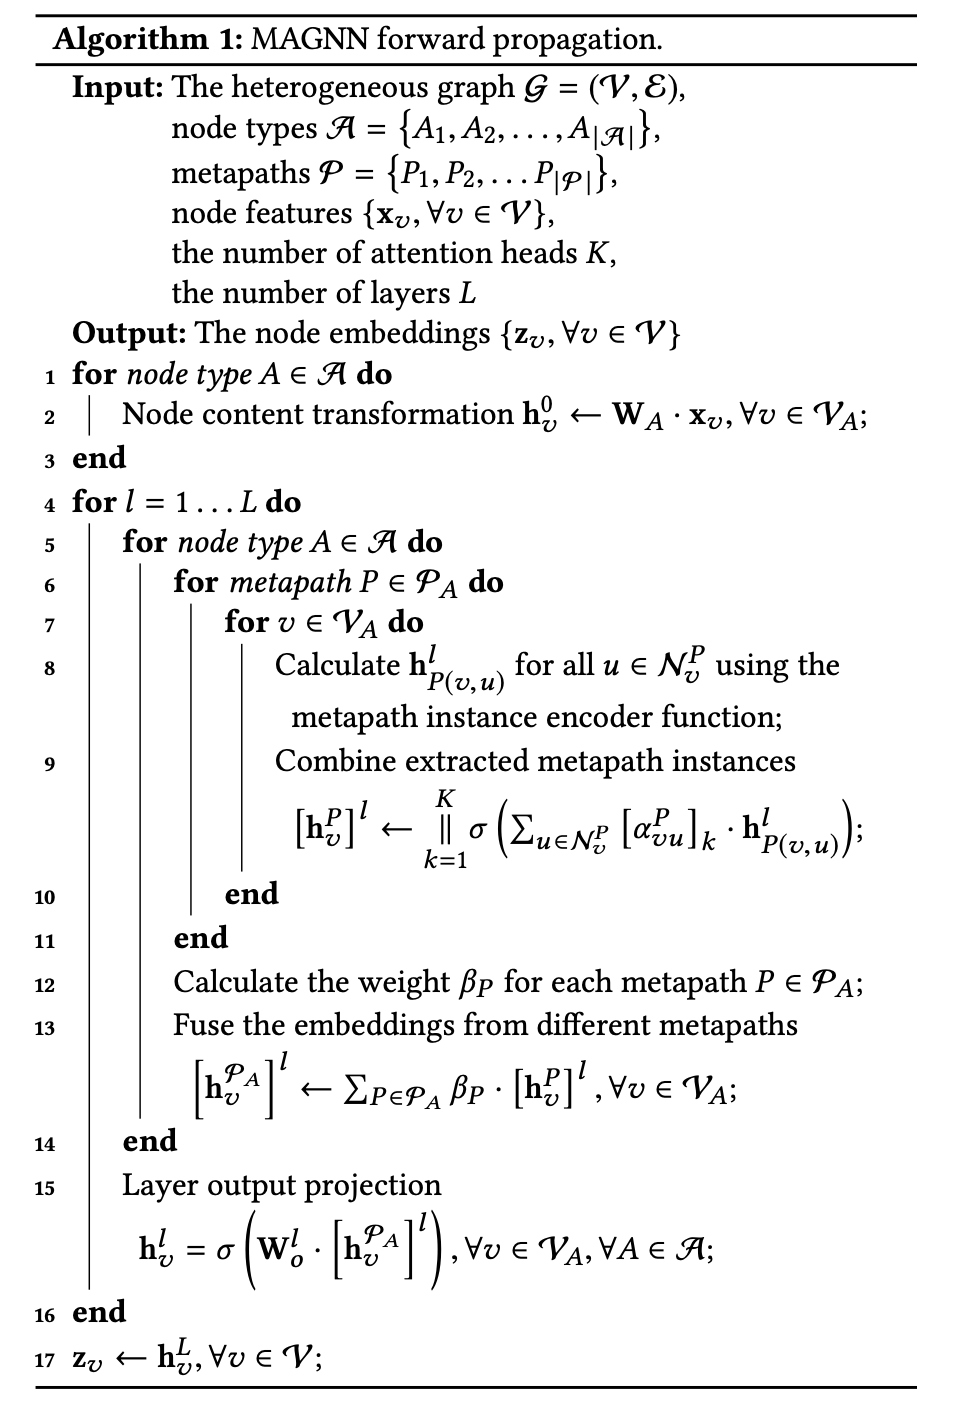
\includegraphics[width=\columnwidth]{figs/alg1.png}
\end{figure}
